Como exemplo para a aplicação de barras de incerteza, continuaremos com os mesmo dados da seção \nameref{sec:reta}, porém agora com as incertezas associadas a cada medida, que foram criadas, novamente, com o auxílio de um computador, e podem ser vistas na figura \ref{fig:incert:dados}.


\subsection{Adicionando Colunas}

    \begin{figure}[htbp]
        \centering
        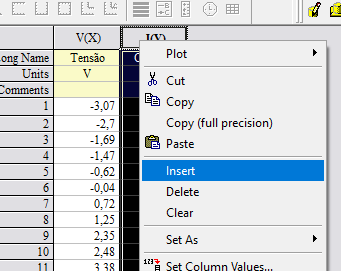
\includegraphics[width=0.4\textwidth]{incert/1insert.png}

        \caption{Inserindo novas colunas}
        \label{fig:incert:colunas}
    \end{figure}

    Para adicionar a incertezas, é preciso gerar novas colunas nas tabelas, como mostra a figura \ref{fig:incert:colunas}, lembrando sempre de formatá-las como na seção \nameref{sec:basico:renome}. A tabela com os dados de incerteza deve ficar algo parecido com a figura \ref{fig:incert:dados}.

    \begin{figure}[htbp]
        \centering
        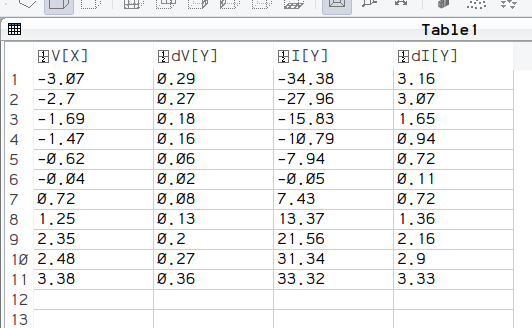
\includegraphics[width=0.5\textwidth]{incert/2dados.png}

        \caption{Dados atualizados com as incertezas}
        \label{fig:incert:dados}
    \end{figure}


\subsection{Tipo das Novas Colunas}

    \begin{figure}[htbp]
        \centering
        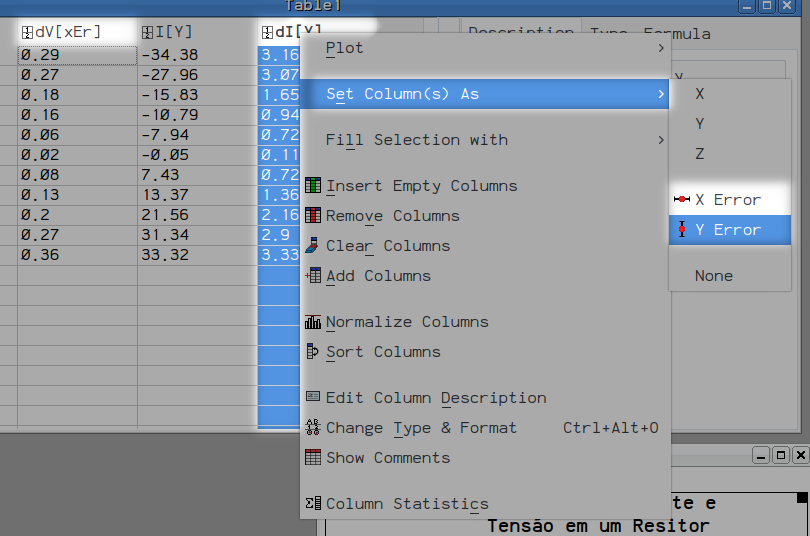
\includegraphics[width=0.6\textwidth]{incert/3xyer.png}
        \caption{Mudando o tipo das novas colunas para relacionar com os valores das medidas}
        \label{fig:incert:tipos}
    \end{figure}


\subsection{Resultados}

    A funcionalidade \texttt{Scatter}, quando selecionada com as colunas de incerteza, gera o gráfico da figura \ref{fig:incert:preresultado}.

    \begin{figure}[htbp]
        \centering
        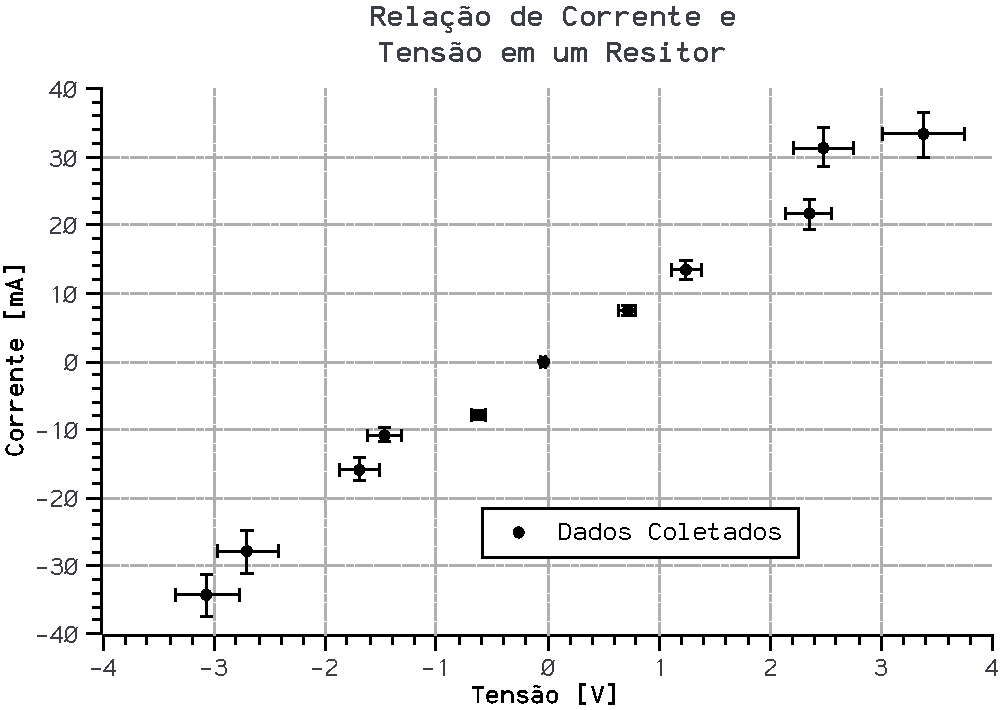
\includegraphics[width=0.6\textwidth]{incert/preresultado.pdf}

        \caption{Gráfico de corrente por tensão com as incertezas de cada medida}
        \label{fig:incert:preresultado}
    \end{figure}

    Entretanto, se for aplicada a formatação da seção \nameref{sec:reta} e a regressão linear, como na seção \nameref{sec:regres}, o resultado deveria ficar semelhante a figura \ref{fig:incert:resultado}, cujos coeficientes são $B = 0.34 \pm 0.11$ e $A = 9.8 \pm 0.3$.

    \begin{figure}[htbp]
        \centering
        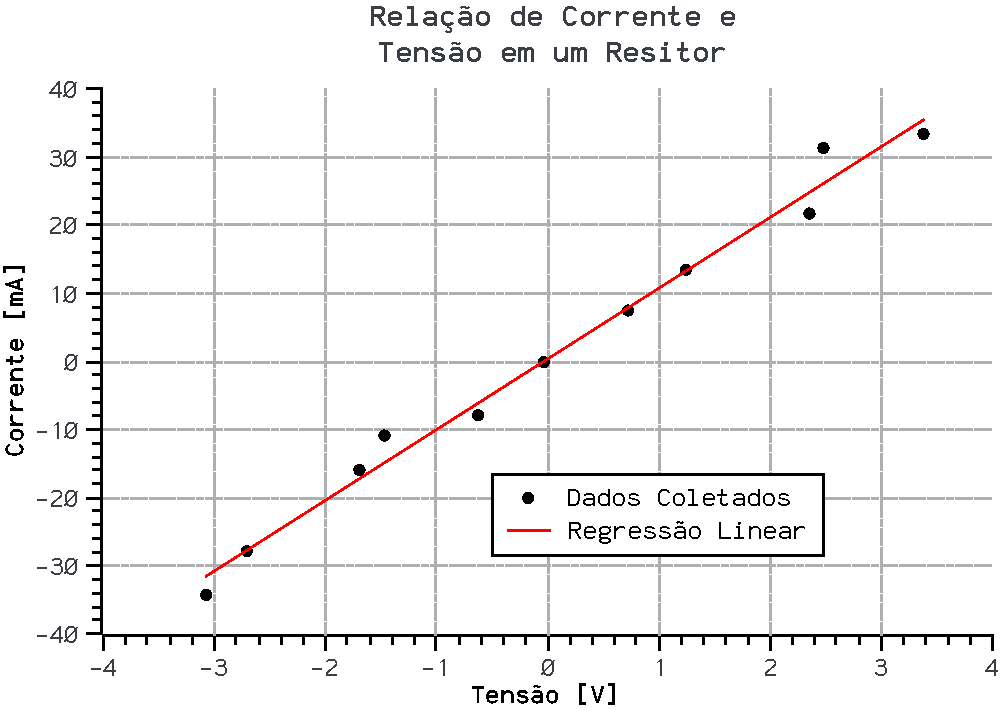
\includegraphics[width=0.6\textwidth]{incert/resultado.pdf}

        \caption{Gráfico formatado, com barras de incerteza e regressão linear}
        \label{fig:incert:resultado}
    \end{figure}

    \begin{nota}
        Note que os coeficientes $A$ e $B$ da regressão em \ref{fig:incert:resultado}, tanto em seus valores quanto nas suas incertezas, são levemente diferentes dos da figura \ref{fig:regres:coefs}, mesmo com os dados numéricos idênticos. A diferença aqui se deve as incertezas dos dados, que agora estão sendo levadas em conta no cálculo da regressão.
    \end{nota}
